\documentclass[11pt,openany]{article}

\usepackage{mathtools, commath}
% Packages for formatting
\usepackage[margin=1in]{geometry}
\usepackage{fancyhdr}
\usepackage{enumerate}
\usepackage{graphicx}
\usepackage{kotex}
\usepackage{amsmath}
\usepackage{amsthm}
\usepackage[dvipsnames,table]{xcolor}
\usepackage{amssymb, amsfonts}

\usepackage{arydshln} % Include this package
% Fonts
\usepackage[T1]{fontenc}
\usepackage[utf8]{inputenc}
\usepackage{newpxtext,newpxmath}
\usepackage{sectsty}

% Define colors
\definecolor{TealBlue1}{HTML}{0077c2}
\definecolor{TealBlue2}{HTML}{00a5e6}
\definecolor{TealBlue3}{HTML}{b3e0ff}
\definecolor{TealBlue4}{HTML}{00293c}
\definecolor{TealBlue5}{HTML}{e6f7ff}

\definecolor{thmcolor}{RGB}{231, 76, 60}
\definecolor{defcolor}{RGB}{52, 152, 219}
\definecolor{lemcolor}{RGB}{155, 89, 182}
\definecolor{corcolor}{RGB}{46, 204, 113}
\definecolor{procolor}{RGB}{241, 196, 15}

\usepackage{color,soul}
\usepackage{soul}
\newcommand{\mathcolorbox}[2]{\colorbox{#1}{$\displaystyle #2$}}
\usepackage{cancel}
\newcommand\crossout[3][black]{\renewcommand\CancelColor{\color{#1}}\cancelto{#2}{#3}}
\newcommand\ncrossout[2][black]{\renewcommand\CancelColor{\color{#1}}\cancel{#2}}

\usepackage{hyperref}
\usepackage{booktabs}

% Chapter formatting
\definecolor{titleTealBlue}{RGB}{0,53,128}
\usepackage{titlesec}
\titleformat{\section}
{\normalfont\sffamily\Large\bfseries\color{titleTealBlue!100!gray}}{\thesection}{1em}{}
\titleformat{\subsection}
{\normalfont\sffamily\large\bfseries\color{titleTealBlue!50!gray}}{\thesubsection}{1em}{}

%Tcolorbox
\usepackage[most]{tcolorbox}
\usepackage{multirow}
\usepackage{multicol}

%Tikzpicture
\usepackage{tikz}
\usepackage{tikz-3dplot}
\usepackage{tikz-cd}
\usetikzlibrary{positioning}
\usetikzlibrary{angles, quotes}
\usetikzlibrary{patterns,patterns.meta}
\usetikzlibrary{decorations.pathreplacing, shapes, arrows}

\usepackage[linesnumbered,ruled]{algorithm2e}
\usepackage{algpseudocode}
\usepackage{setspace}
\SetKwComment{Comment}{/* }{ */}
\SetKwProg{Fn}{Function}{:}{end}
\SetKw{End}{end}
\SetKw{DownTo}{downto}

% Define a new environment for algorithms without line numbers
\newenvironment{algorithm2}[1][]{
	% Save the current state of the algorithm counter
	\newcounter{tempCounter}
	\setcounter{tempCounter}{\value{algocf}}
	% redefine the algorithm numbering (remove prefix)
	\renewcommand{\thealgocf}{}
	\begin{algorithm}
	}{
	\end{algorithm}
	% Restore the algorithm counter state
	\setcounter{algocf}{\value{tempCounter}}
}

\usepackage{adjustbox}
% Header and footer formatting
\pagestyle{fancy}
\fancyhead{}
\fancyhf{}
\rhead{\textcolor{TealBlue2}{\textbf{A Journey from Concretization to Abstraction}}}%\rule{3cm}{0.4pt}}
\lhead{\textcolor{TealBlue2}{\textbf{Abstract Algebra}}}
% Define footer
\newcommand{\footer}[1]{
\begin{flushright}
	\vspace{2em}
	\includegraphics[width=2.5cm]{school_logo.jpg} \\
	\vspace{1em}
	\textcolor{TealBlue2}{\small\textbf{#1}}
\end{flushright}
}
%\rfoot{\large Department of Information Security, Cryptogrphy and Mathematics, Kookmin Uni.\includegraphics[height=1.5cm]{school_logo.jpg}}
\fancyfoot{}
\fancyfoot[C]{-\thepage-}

\newcommand{\ie}{\textnormal{i.e.}}
\newcommand{\rsa}{\mathsf{RSA}}
\newcommand{\rsacrt}{\mathsf{RSA}\textendash\mathsf{CRT}}
\newcommand{\inv}[1]{#1^{-1}}

\usepackage{amsthm}
\newtheorem{axiom}{Axiom}[section]
\newtheorem{theorem}{Theorem}
\newtheorem*{theorem*}{Theorem}
\newtheorem{proposition}[theorem]{Proposition}
\newtheorem{corollary}{Corollary}[theorem]
\newtheorem*{corollary*}{Corollary}
\newtheorem{lemma}[theorem]{Lemma}
\newtheorem*{lemma*}{Lemma}

\theoremstyle{definition}
\newtheorem{definition}{Definition}
\newtheorem*{definition*}{Definition}
\newtheorem*{note}{Note}
\newtheorem{remark}{Remark}
\newtheorem{example}{Example}
\newtheorem{exercise}{Exercise}[section]

%New Command
%\newcommand{\set}[1]{\left\{#1\right\}}
\newcommand{\N}{\mathbb{N}}
\newcommand{\Z}{\mathbb{Z}}
\newcommand{\Q}{\mathbb{Q}}
\newcommand{\R}{\mathbb{R}}
\newcommand{\C}{\mathbb{C}}
\newcommand{\F}{\mathbb{F}}
\newcommand{\nbhd}{\mathcal{N}}
\newcommand{\Log}{\operatorname{Log}}
\newcommand{\Arg}{\operatorname{Arg}}
\newcommand{\pv}{\operatorname{P.V.}}

\newcommand{\of}[1]{\left( #1 \right)} 
%\newcommand{\abs}[1]{\left\lvert #1 \right\rvert}
%\newcommand{\norm}[1]{\left\| #1 \right\|}

\newcommand{\sol}{\textcolor{magenta}{\bf Sol}}
\newcommand{\conjugate}[1]{\overline{#1}}

\newcommand{\res}{\operatorname{res}}
\DeclareMathOperator*{\Res}{\operatorname{Res}}

\renewcommand{\Re}{\operatorname{Re}}
\renewcommand{\Im}{\operatorname{Im}}

\newcommand{\cyclic}[1]{\langle #1 \rangle}
\newcommand{\uniform}{\overset{\$}{\leftarrow}}


\setstretch{1.25}
\begin{document}
\pagenumbering{arabic}
\begin{center}
	\huge\textbf{Equivalence Relations, Equivalence Classes,\\ Partitions, and Quotient Sets}\\
	\vspace{0.5em}
	\Large\quad{Ji, Yong-Hyeon}\\
	\vspace{0.5em}
	\normalsize{\today}\\
\end{center}

\begin{figure}[h!]\centering
\begin{tikzpicture}[scale=1.25]
	% Draw the grid
	\draw[step=1cm,gray,very thin, dotted] (0,0) grid (9.9,9.9);
	
	% Draw the axes
	\draw[thick,->, line width=.5mm] (0,0) -- (10,0) node[anchor=north west] {$a$};
	\draw[thick,->,line width=.5mm] (0,0) -- (0,10) node[anchor=south east] {$b$};
	
	%Take Coordinates
	\foreach \i in {0,1,2,...,9}
	\draw[] (\i,.1)--(\i,-.1) node[below] {$\i$};%x-axis
	\foreach \i in {1,2,...,9}
	\draw[] (.1,\i)--(-.1,\i) node[left] {$\i$};%y-axis
	
	\draw[fill, blue] (0,0) circle (3pt);
	
	% Draw the Relation a = a
	\foreach \x in {0,1,2,...,9} {
		\fill[blue] (\x,\x) circle (3pt);
		\node[anchor=south] at (\x+0.5,\x) {$(a,a)$};
	}
\end{tikzpicture}
\caption{$a=a$ in $\Z\times\Z$}
\end{figure}
\begin{figure}[h!]\centering
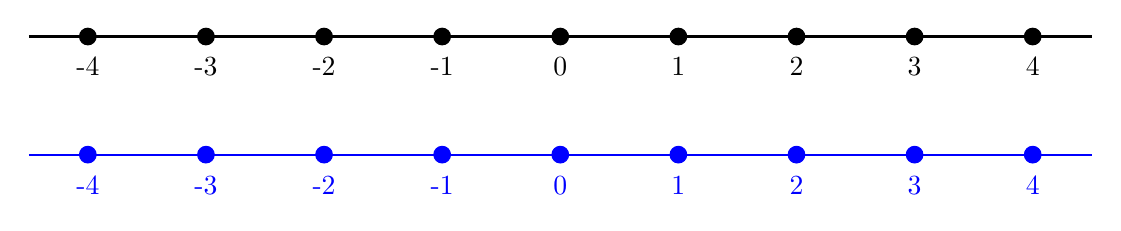
\begin{tikzpicture}[scale=1.5]
	% Draw the main set of integers
	\draw[thick] (-4.5,0) -- (4.5,0);
	\foreach \x in {-4,-3,...,4}
	\filldraw (\x,0) circle (2pt);
	
	% Label the integers
	\foreach \x in {-4,-3,...,4}
	\node[below] at (\x,-.1) {\x};
	
	\draw[thick, blue] (-4.5,-1) -- (4.5,-1);
	\foreach \x in {-4,-3,...,4}
	\filldraw[blue] (\x,-1) circle (2pt);
	
	\foreach \x in {-4,-3,...,4}
	\node[below, blue] at (\x,-1.1) {\x};
\end{tikzpicture}
%	\caption{}
\end{figure}

\begin{figure}[h!]\centering
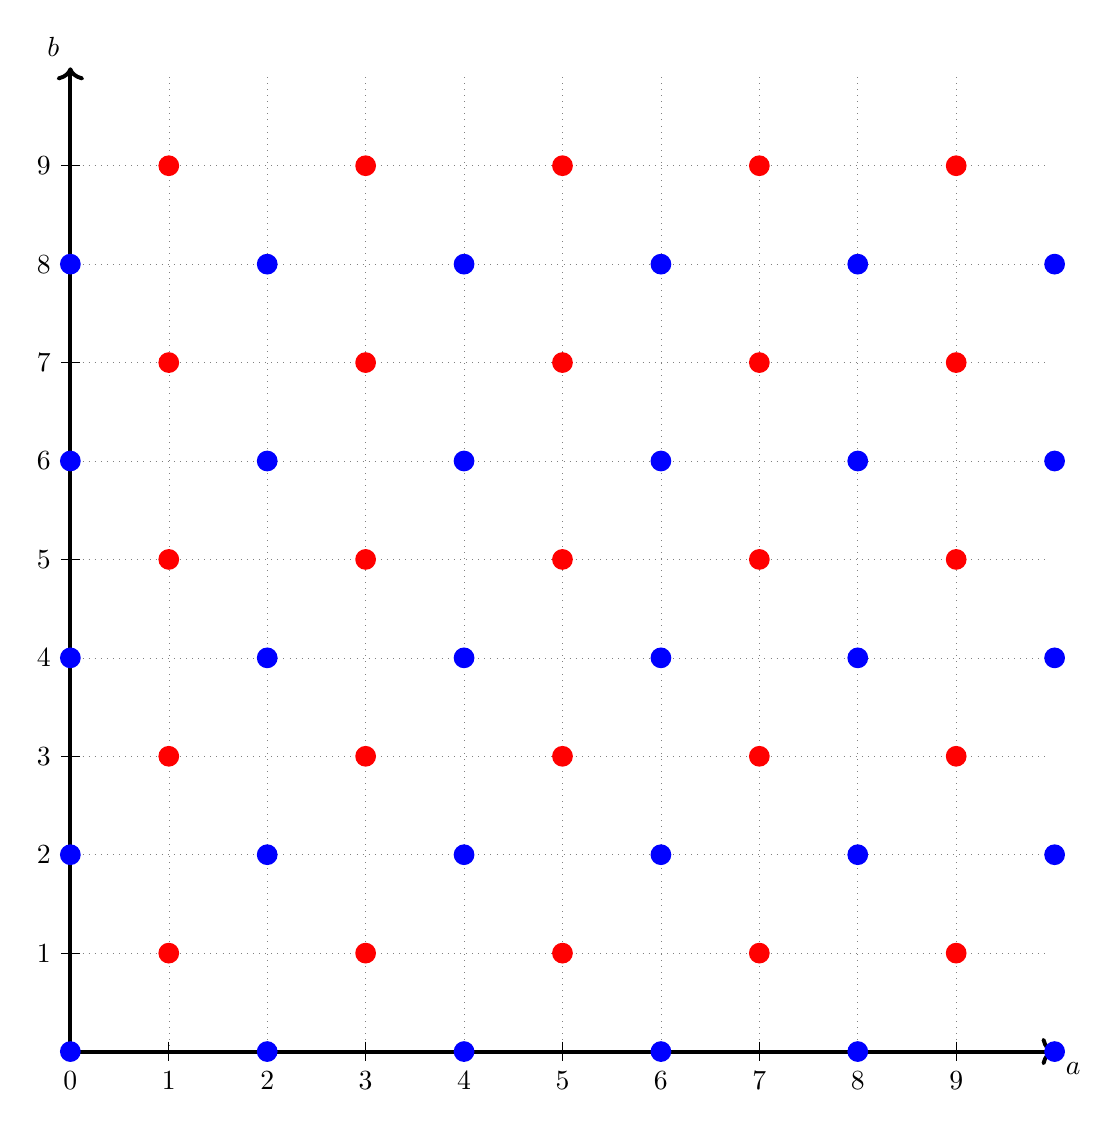
\begin{tikzpicture}[scale=1.25]
	% Draw the grid
	\draw[step=1cm,gray,very thin, dotted] (0,0) grid (9.9,9.9);
	
	% Draw the axes
	\draw[thick,->, line width=.5mm] (0,0) -- (10,0) node[anchor=north west] {$a$};
	\draw[thick,->,line width=.5mm] (0,0) -- (0,10) node[anchor=south east] {$b$};
	
	%Take Coordinates
	\foreach \i in {0,1,2,...,9}
	\draw[] (\i,.1)--(\i,-.1) node[below] {$\i$};%x-axis
	\foreach \i in {1,2,...,9}
	\draw[] (.1,\i)--(-.1,\i) node[left] {$\i$};%y-axis
	
	% Draw the Relation a = 0 (mod 2)
	\foreach \x in {0,2,4,6,8,10}
	\foreach \y in {0,1,...,4} {
		\fill[blue] (\x,2*\y) circle (3pt);
	}
	
	% Draw the Relation a = 1 (mod 2)
	\foreach \x in {1,3,5,7,9}
	\foreach \y in {0,...,4} {
		\fill[red] (\x,2*\y+1) circle (3pt);
	}
\end{tikzpicture}
\caption{$a\equiv b\pmod{2}$ in $\Z\times \Z$}
\end{figure}
\begin{center}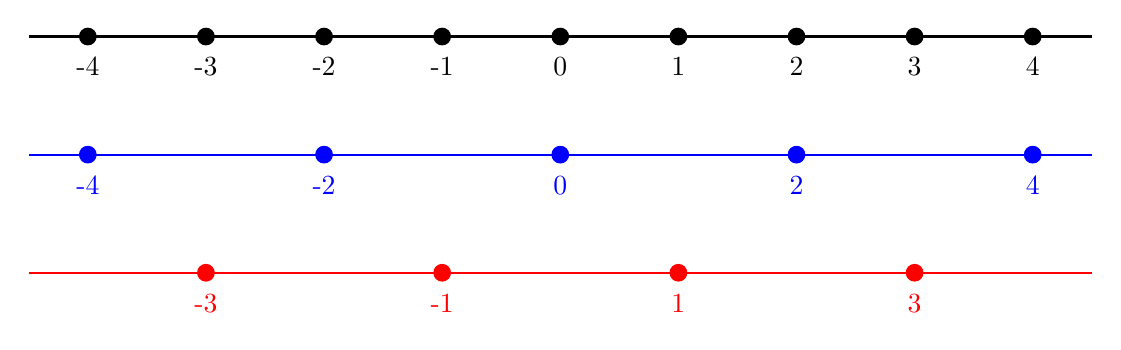
\begin{tikzpicture}[scale=1.5]
	% Draw the main set of integers
	\draw[thick] (-4.5,0) -- (4.5,0);
	\foreach \x in {-4,-3,...,4}
	\filldraw (\x,0) circle (2pt);
	
	% Label the integers
	\foreach \x in {-4,-3,...,4}
	\node[below] at (\x,-.1) {\x};
	
	\draw[thick, blue] (-4.5,-1) -- (4.5,-1);
	\foreach \x in {-4,-2,...,4}
	\filldraw[blue] (\x,-1) circle (2pt);
	
	\foreach \x in {-4,-2,...,4}
	\node[below, blue] at (\x,-1.1) {\x};
	
	\draw[thick, red] (-4.5,-2) -- (4.5,-2);
	\foreach \x in {-3,-1,...,3}
	\filldraw[red] (\x,-2) circle (2pt);
	
	\foreach \x in {-3,-1,...,3}
	\node[below, red] at (\x,-2.1) {\x};
\end{tikzpicture}
\end{center}

\begin{figure}[h!]\centering
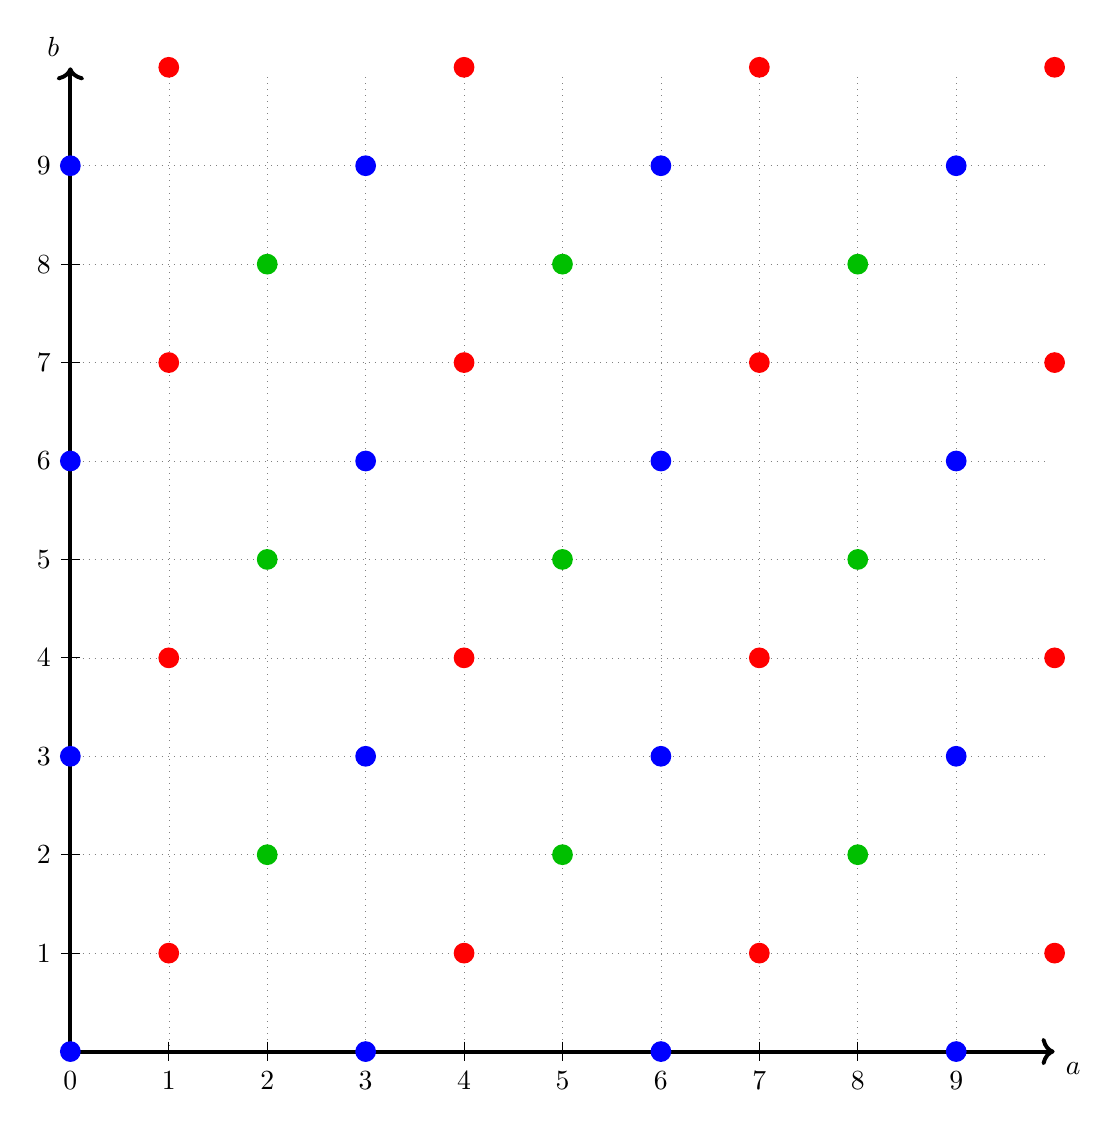
\begin{tikzpicture}[scale=1.25]
	% Draw the grid
	\draw[step=1cm,gray,very thin, dotted] (0,0) grid (9.9,9.9);
	
	% Draw the axes
	\draw[thick,->, line width=.5mm] (0,0) -- (10,0) node[anchor=north west] {$a$};
	\draw[thick,->,line width=.5mm] (0,0) -- (0,10) node[anchor=south east] {$b$};
	
	%Take Coordinates
	\foreach \i in {0,1,2,...,9}
	\draw[] (\i,.1)--(\i,-.1) node[below] {$\i$};%x-axis
	\foreach \i in {1,2,...,9}
	\draw[] (.1,\i)--(-.1,\i) node[left] {$\i$};%y-axis
	
	% Draw the Relation a = 0 (mod 3)
	\foreach \x in {0,3,6,9}
	\foreach \y in {0,1,...,3} {
		\fill[blue] (\x,3*\y) circle (3pt);
	}
	
	% Draw the Relation a = 1 (mod 3)
	\foreach \x in {1,4,...,10}
	\foreach \y in {0,1,...,3} {
		\fill[red] (\x,3*\y+1) circle (3pt);
	}
	
	% Draw the Relation a = 1 (mod 2)
	\foreach \x in {2,5,8}
	\foreach \y in {0,...,2} {
		\fill[green!75!black] (\x,3*\y+2) circle (3pt);
	}
\end{tikzpicture}
\caption{$a\equiv b\pmod{3}$ in $\Z\times \Z$}
\end{figure}
\begin{center}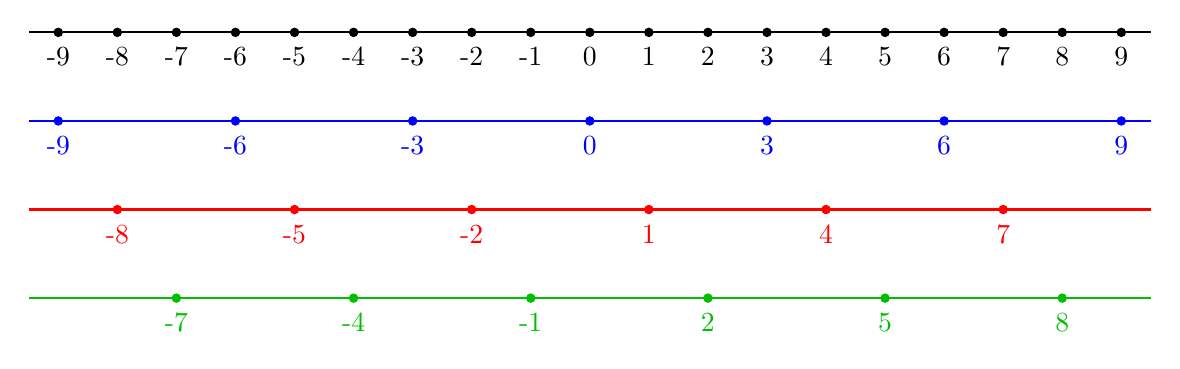
\begin{tikzpicture}[scale=.75]
	% Draw the main set of integers
	\draw[thick] (-9.5,0) -- (9.5,0);
	\foreach \x in {-9,-8,...,9}
	\filldraw (\x,0) circle (2pt);
	
	% Label the integers
	\foreach \x in {-9,-8,...,9}
	\node[below] at (\x,-.1) {\x};
	
	% a = 0 (mod 3)
	\draw[thick, blue] (-9.5,-1.5) -- (9.5,-1.5);
	\foreach \x in {-9,-6,...,9}
	\filldraw[blue] (\x,-1.5) circle (2pt);
	
	\foreach \x in {-9,-6,...,9}
	\node[below, blue] at (\x,-1.6) {\x};
	
	% a = 1 (mod 3)
	\draw[thick, red] (-9.5,-3) -- (9.5,-3);
	\foreach \x in {-8,-5,...,7}
	\filldraw[red] (\x,-3) circle (2pt);
	
	\foreach \x in {-8,-5,...,7}
	\node[below, red] at (\x,-3.1) {\x};
	
	% a = 2 (mod 3)
	\draw[thick, green!75!black] (-9.5,-4.5) -- (9.5,-4.5);
	\foreach \x in {-7,-4,...,8}
	\filldraw[green!75!black] (\x,-4.5) circle (2pt);
	
	\foreach \x in {-7,-4,...,8}
	\node[below, green!75!black] at (\x,-4.6) {\x};
\end{tikzpicture}
\end{center}

\newpage
\begin{center}
\begin{figure}[h!]\centering
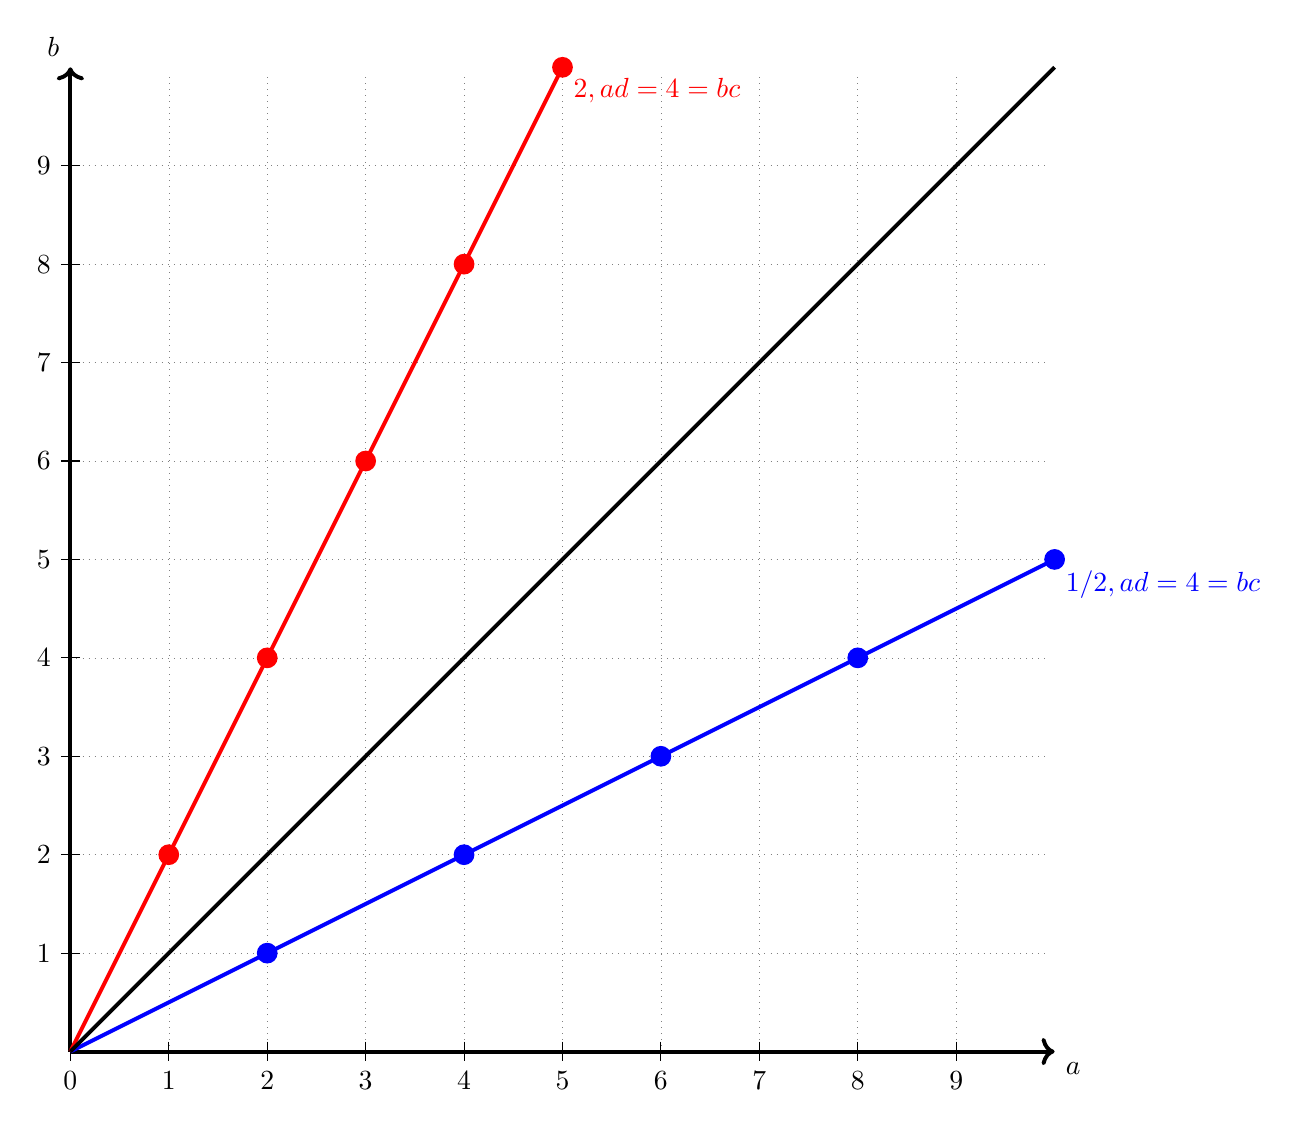
\begin{tikzpicture}[scale=1.25]
	% Draw the grid
	\draw[step=1cm,gray,very thin, dotted] (0,0) grid (9.9,9.9);
	
	% Draw the axes
	\draw[thick,->, line width=.5mm] (0,0) -- (10,0) node[anchor=north west] {$a$};
	\draw[thick,->,line width=.5mm] (0,0) -- (0,10) node[anchor=south east] {$b$};
	
	%Take Coordinates
	\foreach \i in {0,1,2,...,9}
	\draw[] (\i,.1)--(\i,-.1) node[below] {$\i$};%x-axis
	\foreach \i in {1,2,...,9}
	\draw[] (.1,\i)--(-.1,\i) node[left] {$\i$};%y-axis
	
	% Draw the ad=4=bc
	\foreach \x in {1,...,4,5} {
		\fill[blue] (2*\x,\x) circle (3pt);
	}
	\draw[thick,-, line width=.5mm, blue] (0,0) -- (10,5) node[anchor=north west] {$1/2,ad=4=bc$};
	
	% Draw the ad=4=bc
	\foreach \x in {1,...,4,5} {
		\fill[red] (\x,2*\x) circle (3pt);
	}
	\draw[thick,-, line width=.5mm, red] (0,0) -- (5,10) node[anchor=north west] {$2,ad=4=bc$};
	\draw[thick,-, line width=.5mm] (0,0) -- (10,10) node[anchor=north west] {};
\end{tikzpicture}
%	\caption{$a\equiv b\pmod{3}$ in $\Z\times \Z$}
\end{figure}
\end{center}
%\begin{tikzpicture}[scale=1]
%	
%	% Draw grid
%	\draw[step=1cm,gray,very thin] (-6,-6) grid (6,6);
%	
%	% Axes
%	\draw[thick,->] (-6.5,0) -- (6.5,0) node[anchor=north west] {a, c};
%	\draw[thick,->] (0,-6.5) -- (0,6.5) node[anchor=south east] {b, d};
%	
%	% Define colors for different equivalence classes
%	\def\classA{red}
%	\def\classB{blue}
%	\def\classC{green}
%	\def\classD{purple}
%	\def\classE{orange}
%	
%	% Draw points for equivalence classes ad = bc for different products
%	% ad = bc = 1
%	\foreach \a/\b in {-1/1, 1/-1} {
%		\fill[\classA] (\a,\b) circle (3pt);
%		\node[anchor=south east, \classA] at (\a,\b) {(\a,\b)};
%	}
%	
%	% ad = bc = 2
%	\foreach \a/\b in {-2/1, 2/-1} {
%		\fill[\classB] (\a,\b) circle (3pt);
%		\node[anchor=south east, \classB] at (\a,\b) {(\a,\b)};
%	}
%	
%	% ad = bc = 3
%	\foreach \a/\b in {-3/1, 3/-1} {
%		\fill[\classC] (\a,\b) circle (3pt);
%		\node[anchor=south east, \classC] at (\a,\b) {(\a,\b)};
%	}
%	
%	% ad = bc = 4
%	\foreach \a/\b in {-4/1, 4/-1, -2/2, 2/-2} {
%		\fill[\classD] (\a,\b) circle (3pt);
%		\node[anchor=south east, \classD] at (\a,\b) {(\a,\b)};
%	}
%	
%	% ad = bc = 6
%	\foreach \a/\b in {-6/1, 6/-1, -3/2, 3/-2, -2/3, 2/-3} {
%		\fill[\classE] (\a,\b) circle (3pt);
%		\node[anchor=south east, \classE] at (\a,\b) {(\a,\b)};
%	}
%	
%\end{tikzpicture}\\
\begin{figure}[h!]\centering
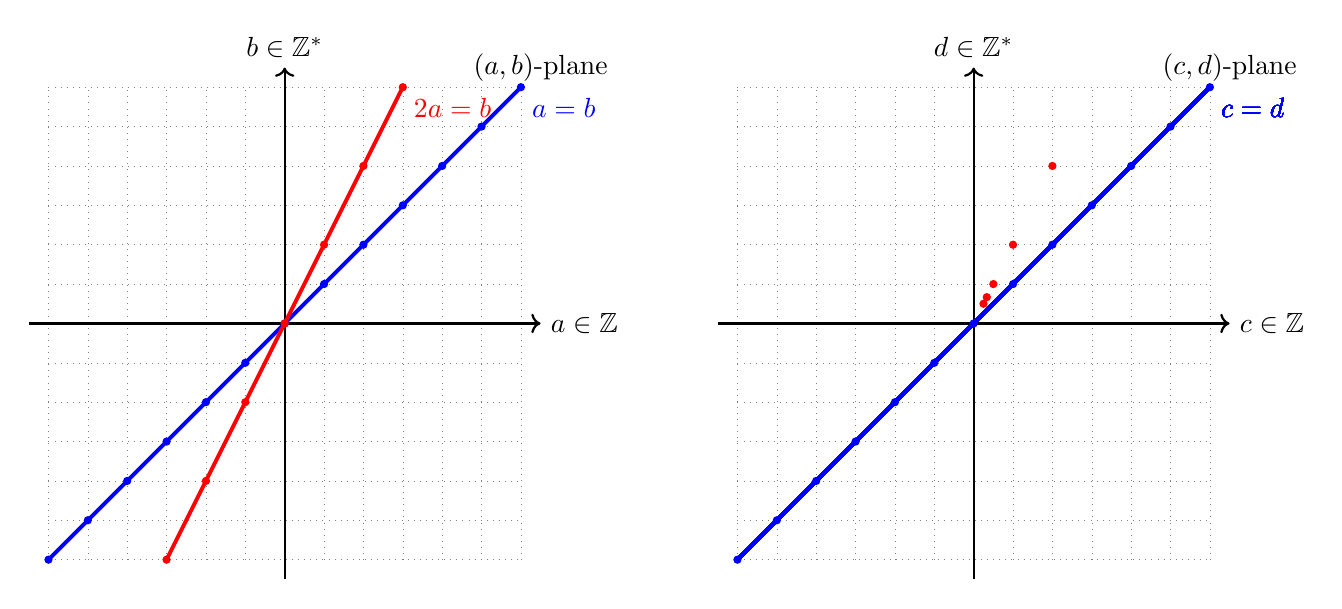
\begin{tikzpicture}[scale=0.5]
	% Draw grid for (a,b) plane
	\draw[step=1cm,gray,very thin, dotted] (-6,-6) grid (6,6);
	% Draw axes for (a,b) plane
	\draw[thick,->] (-6.5,0) -- (6.5,0) node[anchor=west] {$a\in\Z$};
	\draw[thick,->] (0,-6.5) -- (0,6.5) node[anchor=south] {$b\in\Z^*$};
	
	% Label the (a,b) plane
	\node at (6.5, 6.5) {$(a, b)$-plane};
	
	% Draw grid for (c,d) plane
	\begin{scope}[xshift=17.5cm]
		\draw[step=1cm,gray,very thin,dotted] (-6,-6) grid (6,6);
		% Draw axes for (c,d) plane
		\draw[thick,->] (-6.5,0) -- (6.5,0) node[anchor=west] {$c\in\Z$};
		\draw[thick,->] (0,-6.5) -- (0,6.5) node[anchor=south] {$d\in\Z^*$};
		
		% Label the (c,d) plane
		\node at (6.5, 6.5) {$(c, d)$-plane};
	\end{scope}
	
	% Define points and colors for equivalence classes
	\def\classColorA{red}
	\def\classColorB{blue}
	\def\classColorC{green}
	
%	\foreach \a/\b in {1/6, 2/3, 3/2, 6/1, -1/-6, -2/-3, -3/-2, -6/-1} {
%		\fill[\classColorA] (\a,\b) circle (3pt);
%		\node[anchor=south east, \classColorA] at (\a,\b) {(\a,\b)};
%	}
	\foreach \x in {-6,...,6} {
		\fill[blue] (\x,\x) circle (3pt);
	}
	\draw[thick,-, line width=.5mm, blue] (-6,-6) -- (6,6) node[anchor=north west] {$a=b$};
	
	\foreach \x in {-3,...,3} {
		\fill[red] (\x,2*\x) circle (3pt);
	}
	\draw[thick,-, line width=.5mm, red] (-3,-6) -- (3,6) node[anchor=north west] {$2a=b$};
	
	\begin{scope}[xshift=17.5cm]
		\fill[red] (1,2) circle (3pt);
		\fill[red] (2,4) circle (3pt);
		\fill[red] (1/2,1) circle (3pt);
		\fill[red] (1/3,2/3) circle (3pt);
		\fill[red] (1/4,1/2) circle (3pt);
	\end{scope}
	
	\foreach \x in {-6,...,6} {
		\begin{scope}[xshift=17.5cm]
			\fill[blue] (\x,\x) circle (3pt);
			\draw[thick,-, line width=.5mm, blue] (-6,-6) -- (6,6) node[anchor=north west] {$c=d$};
		\end{scope}	
	}
%	\draw[\classColorA, thick, arrows=-Stealth, dotted, bend angle=15] (1/2,1/2) -- (21.5,4);
%	\draw[\classColorA, thick, arrows=-Stealth, dotted, bend angle=15] (1,1) -- (19.5,2);
%	\draw[\classColorA, thick, arrows=-Stealth, dotted, bend angle=15] (2,2) -- (18.5,1);
	
%	\fill[red] (1,2) circle (3pt);
%	\fill[red] (18.5,1) circle (3pt);
	% Points for ad = bc = 6
%	\foreach \a/\b in {1/6, 2/3, 3/2, 6/1, -1/-6, -2/-3, -3/-2, -6/-1} {
%		\fill[\classColorA] (\a,\b) circle (3pt);
%		\node[anchor=south east, \classColorA] at (\a,\b) {(\a,\b)};
%	}
%	
%	\foreach \c/\d in {1/6, 2/3, 3/2, 6/1, -1/-6, -2/-3, -3/-2, -6/-1} {
%		\begin{scope}[xshift=15cm]
%			\fill[\classColorA] (\c,\d) circle (3pt);
%			\node[anchor=south east, \classColorA] at (\c,\d) {(\c,\d)};
%		\end{scope}
%	}
%	
%	% Example connecting lines for equivalence class ad = bc = 6
%	\draw[\classColorA, thick, dashed] (1,6) -- ++(15cm,0);
%	\draw[\classColorA, thick, dashed] (2,3) -- ++(15cm,0);
%	\draw[\classColorA, thick, dashed] (3,2) -- ++(15cm,0);
%	\draw[\classColorA, thick, dashed] (6,1) -- ++(15cm,0);
	
	% Additional points and connections for other equivalence classes can be added similarly
	% e.g., for ad = bc = 12, 18, etc., following the same pattern
\end{tikzpicture}
\caption{$ad=bc=2$}
\end{figure}

\newpage
\section{Introduction}
This document explores the concepts of equivalence relations, partitioning, and quotient sets by observing and analyzing patterns within the set of integers, \( \mathbb{Z} \). We begin with intuitive observations and gradually formalize these into rigorous mathematical definitions.

\section{Natural Observations}
Consider the set of all integers \( \mathbb{Z} \). An initial observation might note that integers can be grouped based on their remainders when divided by a certain number, say \( n \). This leads to an intuitive grouping based on shared properties.

\subsection{Grouping by Remainders}
When we divide integers by 2, for instance, every integer falls into one of two categories: even or odd. This division is based on the remainder of the division:
\begin{itemize}
	\item Even integers (\(0, 2, 4, -2, -4, \dots\)) have a remainder of 0.
	\item Odd integers (\(1, 3, 5, -1, -3, \dots\)) have a remainder of 1.
\end{itemize}

\section{Formalizing Observations into Equivalence Relations}
The observed grouping suggests a relation among integers based on their remainders when divided by a number \( n \). We define an equivalence relation \( \sim \) on \( \mathbb{Z} \) as follows:

\subsection{Definition of Equivalence Relation}
A relation \( \sim \) on \( \mathbb{Z} \) is called an equivalence relation if it satisfies the following properties:
\begin{itemize}
	\item \textbf{Reflexivity}: \( a \sim a \)
	\item \textbf{Symmetry}: If \( a \sim b \) then \( b \sim a \)
	\item \textbf{Transitivity}: If \( a \sim b \) and \( b \sim c \) then \( a \sim c \)
\end{itemize}

For our example, define \( a \sim b \) iff \( a \equiv b \pmod{n} \).

\section{Partitioning of Integers}
Given our equivalence relation, we can partition \( \mathbb{Z} \) into disjoint subsets, where each subset contains integers that are equivalent under \( \sim \).

\subsection{Equivalence Classes}
Each subset, known as an equivalence class, includes all integers sharing the same remainder when divided by \( n \). The set of all equivalence classes is given by:
\[
\{[a] \mid a \in \mathbb{Z}\}, \text{ where } [a] = \{b \in \mathbb{Z} \mid b \equiv a \pmod{n}\}
\]

\section{Quotient Set}
The collection of all such equivalence classes forms a quotient set, denoted as \( \mathbb{Z}/n\mathbb{Z} \), which simplifies the study of integers by focusing on the structure of these classes rather than individual elements.

\section{Conclusion}
Through the example of integers, we have seen how natural observations can lead to the formal mathematical concepts of equivalence relations, partitioning, and quotient sets, providing a structured way to analyze and simplify complex sets.
\begin{figure}[h!]
	\centering
	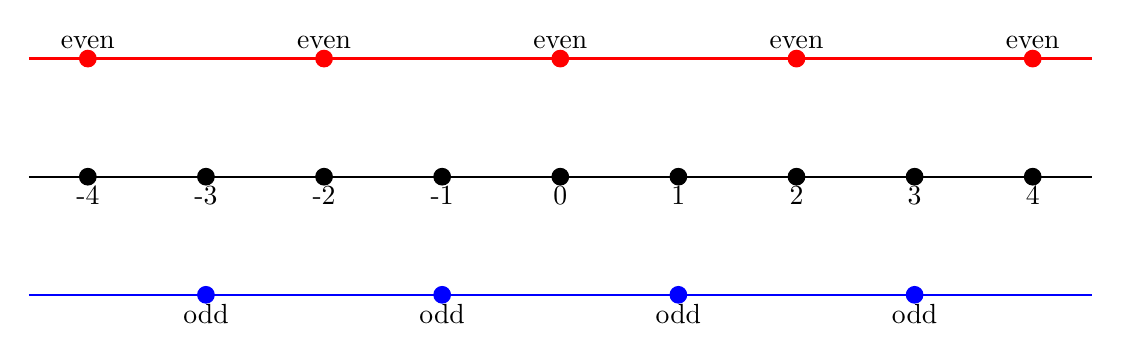
\begin{tikzpicture}[scale=1.5]
		% Draw the main set of integers
		\draw[thick] (-4.5,0) -- (4.5,0);
		\foreach \x in {-4,-3,...,4}
		\filldraw (\x,0) circle (2pt);
		
		% Label the integers
		\foreach \x in {-4,-3,...,4}
		\node[below] at (\x,0) {\x};
		
		% Draw partitions for mod 2
		\draw[thick, red] (-4.5,1) -- (4.5,1);
		\foreach \x in {-4,-2,...,4}
		\filldraw[red] (\x,1) circle (2pt);
		
		\foreach \x in {-4,-2,...,4}
		\node[above] at (\x,1) {even};
		
		\draw[thick, blue] (-4.5,-1) -- (4.5,-1);
		\foreach \x in {-3,-1,...,3}
		\filldraw[blue] (\x,-1) circle (2pt);
		
		\foreach \x in {-3,-1,...,3}
		\node[below] at (\x,-1) {odd};
		
		% Add labels for equivalence classes
%		\node[red, above] at (0, 1.5) {Equivalence Class $[0]$};
%		\node[blue, below] at (0, -1.5) {Equivalence Class $[1]$};
%		
%		% Draw brackets for equivalence classes
%		\draw[decorate,decoration={brace,amplitude=10pt,mirror,raise=4pt},yshift=0pt]
%		(-4.5,1.5) -- (4.5,1.5) node [black,midway,yshift=0.6cm] {};
%		
%		\draw[decorate,decoration={brace,amplitude=10pt,raise=4pt},yshift=0pt]
%		(-4.5,-1.5) -- (4.5,-1.5) node [black,midway,yshift=-0.6cm] {};
	\end{tikzpicture}
	\caption{Illustration of Equivalence Classes and Partitioning of Integers Modulo 2}
	\label{fig:equiv_classes}
\end{figure}
\newpage

\section{Introduction}
In this seminar, we explore foundational concepts of group theory and ring theory through intuitive examples within the set of integers, \( \mathbb{Z} \). We focus on naturally deriving the definitions of normal subgroups and various types of ideals.

\section{Group-Theoretic Concepts}
We begin with basic observations about the integers under addition and their subgroup structures.

\subsection{Subgroups and Normal Subgroups}
Consider the set of integers \( \mathbb{Z} \) under addition. Subgroups of \( \mathbb{Z} \) are subsets that are closed under addition and have additive inverses. For example, the set of even integers, \( 2\mathbb{Z} \), forms a subgroup.

\subsubsection{Observation of Normality}
Notice that in \( \mathbb{Z} \), not only is \( 2\mathbb{Z} \) a subgroup, but it is also normal because integer addition is commutative:
\[
a + b = b + a, \quad \forall a, b \in \mathbb{Z}
\]
Thus, any subgroup of \( \mathbb{Z} \) is normal, since subgroup elements commute with all elements of \( \mathbb{Z} \).

\section{Ring-Theoretic Concepts}
Next, we consider \( \mathbb{Z} \) as a ring, and observe properties that lead to the definitions of ideals.

\subsection{Ideals of a Ring}
An ideal in \( \mathbb{Z} \) is a subset closed under addition and absorption by multiplication from \( \mathbb{Z} \). The set \( n\mathbb{Z} \) for any integer \( n \) is an example of an ideal.

\subsubsection{Prime and Maximal Ideals}
\paragraph{Prime Ideals}
An ideal \( I \) in a ring \( R \) is prime if for any elements \( a, b \) in \( R \), \( ab \in I \) implies \( a \in I \) or \( b \in I \). In \( \mathbb{Z} \), the ideal generated by a prime number \( p \), \( p\mathbb{Z} \), is a prime ideal. For instance:
\[
3\mathbb{Z} \text{ is prime because if } ab \in 3\mathbb{Z}, \text{ then either } a \text{ or } b \text{ is divisible by } 3.
\]

\paragraph{Maximal Ideals}
An ideal \( I \) is maximal if there is no other ideal \( J \) such that \( I \subset J \subset R \). In \( \mathbb{Z} \), \( p\mathbb{Z} \) is also maximal if \( p \) is a prime number, because the quotient \( \mathbb{Z}/p\mathbb{Z} \) is a field.

\section{Conclusion}
Through intuitive observations within the set of integers, we have derived significant algebraic concepts such as normal subgroups and different types of ideals. This approach not only simplifies understanding but also demonstrates the practical applications and implications of these concepts in abstract algebra.

\begin{figure}[h!]
	\centering
	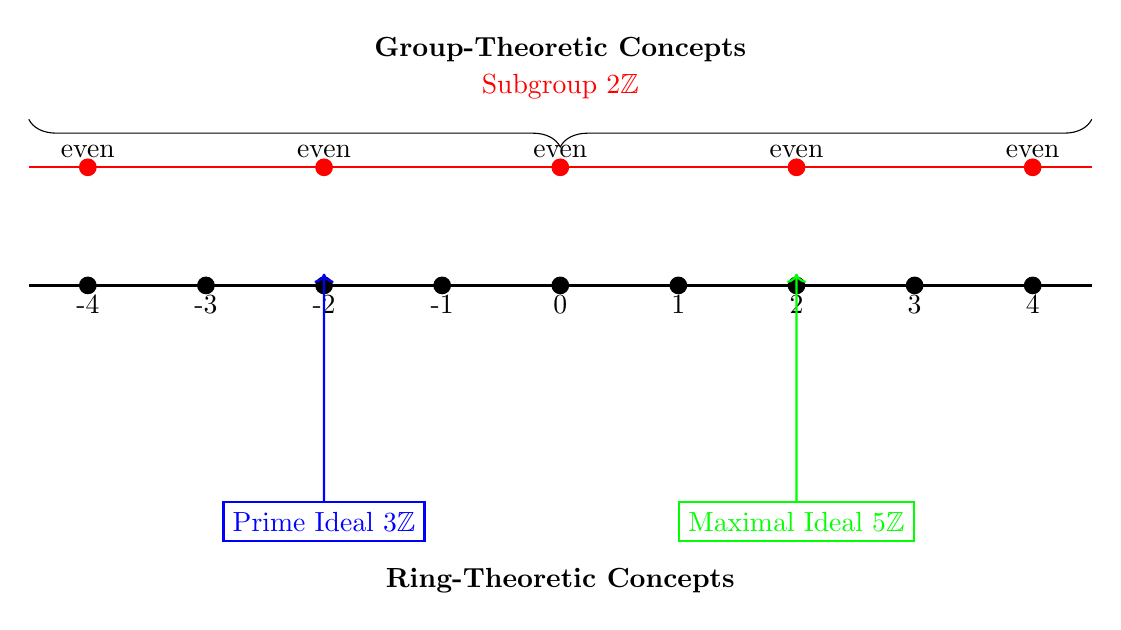
\begin{tikzpicture}[scale=1.5]
		% Draw the main set of integers
		\draw[thick] (-4.5,0) -- (4.5,0);
		\foreach \x in {-4,-3,...,4}
		\filldraw (\x,0) circle (2pt);
		
		% Label the integers
		\foreach \x in {-4,-3,...,4}
		\node[below] at (\x,0) {\x};
		
		% Draw subgroups for 2Z (even integers)
		\draw[thick, red] (-4.5,1) -- (4.5,1);
		\foreach \x in {-4,-2,...,4}
		\filldraw[red] (\x,1) circle (2pt);
		
		\foreach \x in {-4,-2,...,4}
		\node[above] at (\x,1) {even};
		
		% Labels for subgroups
		\node[red, above] at (0, 1.5) {Subgroup $2\mathbb{Z}$};
		
		% Draw brackets for normal subgroup
		\draw[decorate,decoration={brace,amplitude=10pt,mirror,raise=4pt},yshift=0pt]
		(-4.5,1.5) -- (4.5,1.5);
		
		% Ring-Theoretic Concepts (Ideals)
		% Prime ideal example
		\node[draw, thick, rectangle, minimum width=2cm, minimum height=0.5cm, blue] (primeideal) at (-2,-2) {Prime Ideal $3\mathbb{Z}$};
		\draw[thick, ->, blue] (primeideal.north) -- (-2,0.1);
		
		% Maximal ideal example
		\node[draw, thick, rectangle, minimum width=2cm, minimum height=0.5cm, green] (maxideal) at (2,-2) {Maximal Ideal $5\mathbb{Z}$};
		\draw[thick, ->, green] (maxideal.north) -- (2,0.1);
		
		% Caption for Group-Theoretic Concepts
		\node at (0, 2) {\textbf{Group-Theoretic Concepts}};
		
		% Caption for Ring-Theoretic Concepts
		\node at (0, -2.5) {\textbf{Ring-Theoretic Concepts}};
	\end{tikzpicture}
	\caption{Illustration of Subgroups, Normal Subgroups, and Ideals within \( \mathbb{Z} \)}
	\label{fig:algebra_concepts}
\end{figure}

\newpage
%\begin{tikzpicture}[scale=1.5]
%	
%	% Draw the outer circle representing group G
%	\draw[thick] (0,0) circle (3cm);
%	\node at (0,3.2) {$G$};
%	
%	% Draw the inner circle representing the normal subgroup N
%	\draw[thick] (0,0) circle (1.5cm);
%	\node at (0,1.7) {$N$};
%	
%	% Draw elements of G
%	\foreach \angle in {0,45,...,315}
%%	\filldraw (3cm*\angle:1pt) circle (2pt);
%	
%	% Draw elements of N
%	\foreach \angle in {0,90,...,270}
%	\filldraw (1.5cm*\angle:1pt) circle (2pt);
%	
%	% Draw arrows indicating normal subgroup property
%%	\foreach \angle in {0,90,...,270} {
%%		\draw[->,thick] (1.5cm*\angle:1.5cm) -- (3cm*\angle:3cm);
%%		\draw[->,thick] (3cm*\angle:3cm) -- (1.5cm*\angle:1.5cm);
%%	}
%	
%	% Draw label for G and N
%	\node at (0,0) {$e$};
%	
%	% Draw cosets
%	\node at (1.5, 0) {$gN$};
%	\node at (-1.5, 0) {$hN$};
%	
%\end{tikzpicture}
%\begin{thebibliography}{99}

%\bibitem{schlenga2020cdcl}
%Schlenga, Alexander T. (2020). "Conflict Driven Clause Learning". June 8, 2020.

\bibitem{HankersonMenezesVanstone}
Darrel Hankerson, Alfred Menezes, and Scott Vanstone.
\newblock \emph{Guide to Elliptic Curve Cryptography}.
\newblock Springer-Verlag, New York, 2004.

\end{thebibliography}

\end{document}
